105. \begin{figure}[ht!]
\center{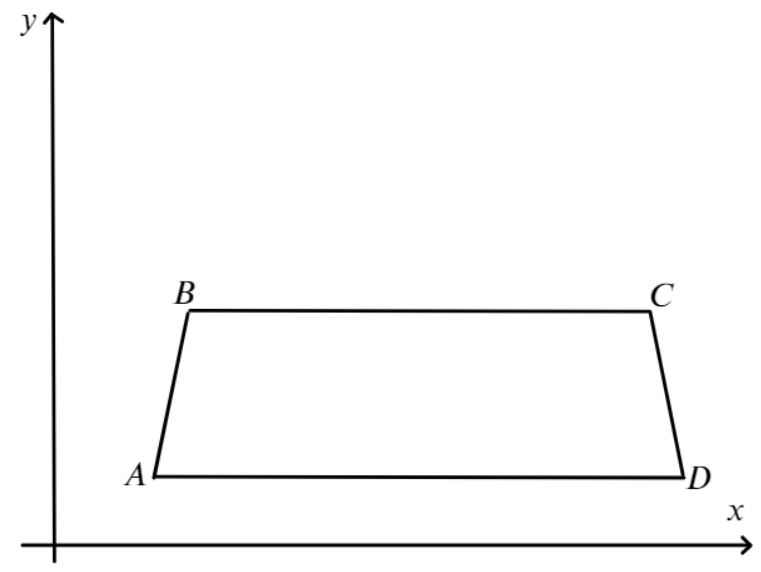
\includegraphics[scale=0.35]{g9-105.png}}
\end{figure}\\
Если трапеция вписанная, то она равнобедренная. Так как абсцисса точки $B$ на 1 больше абсциссы точки $A,$ абсцисса точки $D$ должна быть на 1 больше абсциссы точки $C,$ то есть $D$ имеет координаты $(17;2).$ Высота трапеции равна $7-2=5,$ значит $S_{ABCD}=5\cdot\cfrac{(17-3)+(16-4)}{2}=65.$\newpage\noindent
